% Hlavicka pro protokoly z fyzikalniho praktika.
% Verze pro: LaTeX
% Verze hlavicky: 22. 2. 2007
% Autor: Ustav fyziky kondenzovanych latek
% Ke stazeni: www.physics.muni.cz/ufkl/Vyuka/
% Licence: volne k pouziti, nejlepe k vcasnemu odevzdani protokolu z Vaseho mereni.


\documentclass[english,11pt,a4paper]{article}
\usepackage[T1]{fontenc}
\usepackage{graphicx, animate}
\usepackage{mathtools}
\usepackage{amssymb}
\usepackage{amsthm}
\usepackage{thmtools}
\usepackage{xcolor}
\usepackage{nameref}
\usepackage{babel}
\usepackage{hyperref}
\usepackage{multicol}
\usepackage[export]{adjustbox}
\usepackage{subcaption}
\usepackage{caption}
\usepackage{multirow}
\usepackage{float}
\usepackage{placeins}
\graphicspath{ {./images/} }

\usepackage[backend=biber,style=numeric]{biblatex}       % [1], [2], ...


\addbibresource{ref.bib}

%%% Nemente:
\usepackage[margin=2cm]{geometry}
\newtoks\jmenopraktika \newtoks\jmeno \newtoks\datum
\newtoks\obor \newtoks\skupina \newtoks\rocnik \newtoks\semestr
\newtoks\cisloulohy \newtoks\jmenoulohy
\newtoks\tlak \newtoks\teplota \newtoks\vlhkost
%%% Nemente - konec.


%%%%%%%%%%% Doplnte pozadovane polozky:

\jmenopraktika={Physical laboratory 3}  % nahradte jmenem vaseho predmetu
\jmeno={Teodor Duraković}            % nahradte jmenem mericiho
\datum={1.~april 2025}        % nahradte datem mereni ulohy
\obor={F}                     % nahradte zkratkou vami studovaneho oboru
\skupina={Út 14:00}            % nahradte dobou vyuky vasi seminarni skupiny
\rocnik={II}                  % nahradte rocnikem, ve kterem studujete
\semestr={IV}                 % nahradte semestrem, ve kterem studujete

\cisloulohy={8}               % nahradte cislem merene ulohy
\jmenoulohy={Band gap width} % nahradte jmenem merene ulohy

\tlak={983}                   % nahradte tlakem pri mereni (v hPa)
\teplota={20.2}               % nahradte teplotou pri mereni (ve stupnich Celsia)
\vlhkost={35}               % nahradte vlhkosti vzduchu pri mereni (v %)

%%%%%%%%%%% Konec pozadovanych polozek.


%%%%%%%%%%% Uzitecne balicky:

%%%%%% Zamezeni parchantu:
\widowpenalty 10000 \clubpenalty 10000 \displaywidowpenalty 10000
%%%%%% Parametry pro moznost vsazeni vetsiho poctu obrazku na stranku
\setcounter{topnumber}{3}	  % max. pocet floatu nahore (specifikace t)
\setcounter{bottomnumber}{3}	  % max. pocet floatu dole (specifikace b)
\setcounter{totalnumber}{6}	  % max. pocet floatu na strance celkem
\renewcommand\topfraction{0.9}	  % max podil stranky pro floaty nahore
\renewcommand\bottomfraction{0.9} % max podil stranky pro floaty dole
\renewcommand\textfraction{0.1}	  % min podil stranky, ktery musi obsahovat text
\intextsep=8mm \textfloatsep=8mm  %\intextsep pro ulozeni [h] floatu a \textfloatsep pro [b] or [t]

% Tecky za cisly sekci:
\renewcommand{\thesection}{\arabic{section}.}
\renewcommand{\thesubsection}{\thesection\arabic{subsection}.}
\renewcommand{\thesubsubsection}{\thesubsection\arabic{subsubsection}.}
% Jednopismenna mezera mezi cislem a nazvem kapitoly:
\makeatletter \def\@seccntformat#1{\csname the#1\endcsname\hspace{1ex}} \makeatother


%%%%%%%%%%%%%%%%%%%%%%%%%%%%%%%%%%%%%%%%%%%%%%%%%%%%%%%%%%%%%%%%%%%%%%%%%%%%%%%
%%%%%%%%%%%%%%%%%%%%%%%%%%%%%%%%%%%%%%%%%%%%%%%%%%%%%%%%%%%%%%%%%%%%%%%%%%%%%%%
% Zacatek dokumentu
%%%%%%%%%%%%%%%%%%%%%%%%%%%%%%%%%%%%%%%%%%%%%%%%%%%%%%%%%%%%%%%%%%%%%%%%%%%%%%%
%%%%%%%%%%%%%%%%%%%%%%%%%%%%%%%%%%%%%%%%%%%%%%%%%%%%%%%%%%%%%%%%%%%%%%%%%%%%%%%

\begin{document}
	
	%%%%%%%%%%%%%%%%%%%%%%%%%%%%%%%%%%%%%%%%%%%%%%%%%%%%%%%%%%%%%%%%%%%%%%%%%%%%%%%
	% Nemente:
	%%%%%%%%%%%%%%%%%%%%%%%%%%%%%%%%%%%%%%%%%%%%%%%%%%%%%%%%%%%%%%%%%%%%%%%%%%%%%%%
	\thispagestyle{empty}
	
	{
		\begin{center}
			\sf 
			{\Large Department of Plasma Physics and Technology} \\
			\bigskip
			{\huge \bfseries PHYSICAL LABORATORY 3} \\
			\bigskip
			{\Large \the\jmenopraktika}
		\end{center}
		
		\bigskip
		
		\sf
		\noindent
		\setlength{\arrayrulewidth}{1pt}
		\begin{tabular*}{\textwidth}{@{\extracolsep{\fill}} l l}
			\large {\bfseries Processed by:}  \the\jmeno & \large  {\bfseries Measured:} \the\datum\\[2mm]
			\large  {\bfseries Field:} \the\obor  \hspace{40mm}  {\bfseries Group:} \the\skupina %
			%{\bfseries Ročník:} \the\rocnik \hspace{5mm} {\bfseries Semestr:} \the\semestr  
			&\large {\bfseries Tested:}\\
			\\
			\hline
		\end{tabular*}
	}
	
	\bigskip
	
	{
		\sf
		\noindent \begin{tabular}{p{3cm} p{0.6\textwidth}}
			\Large  Task № {\bfseries \the\cisloulohy:} \par
			&\Large \bfseries \the\jmenoulohy  \\[2mm]
		\end{tabular}
	}
	
	\vskip1cm
	
	%%%%%%%%%%%%%%%%%%%%%%%%%%%%%%%%%%%%%%%%%%%%%%%%%%%%%%%%%%%%%%%%%%%%%%%%%%%%%%%
	% konec Nemente.
	%%%%%%%%%%%%%%%%%%%%%%%%%%%%%%%%%%%%%%%%%%%%%%%%%%%%%%%%%%%%%%%%%%%%%%%%%%%%%%%
	
	%%%%%%%%%%%%%%%%%%%%%%%%%%%%%%%%%%%%%%%%%%%%%%%%%%%%%%%%%%%%%%%%%%%%%%%%%%%%%%%
	%%%%%%%%%%%%%%%%%%%%%%%%%%%%%%%%%%%%%%%%%%%%%%%%%%%%%%%%%%%%%%%%%%%%%%%%%%%%%%%
	% Zacatek textu vlastniho protokolu
	%%%%%%%%%%%%%%%%%%%%%%%%%%%%%%%%%%%%%%%%%%%%%%%%%%%%%%%%%%%%%%%%%%%%%%%%%%%%%%%
	%%%%%%%%%%%%%%%%%%%%%%%%%%%%%%%%%%%%%%%%%%%%%%%%%%%%%%%%%%%%%%%%%%%%%%%%%%%%%%%
	
	\begin{multicols}{2}
		\section{Tasks}
	
	1. Determine the energy band gap of silicon and germanium using the photoelectrict effect.

		\section{Theory}
		
		Solid-state materials can be classified as conductors, semiconductors, or insulators, based on the structure of their electronic energy bands. In semiconductors, the valence band (filled with electrons) and the conduction band (empty at $0\,\mathrm{K}$) are separated by a relatively narrow forbidden band gap $E_g$. At room temperature, a small number of electrons gain sufficient thermal energy to transition from the valence band to the conduction band, becoming mobile charge carriers. This process also leaves mobile “holes” in the valence band behind.
		
		The width of the band gap $E_g$ is a fundamental property of semiconductors, as it determines the material's electrical and optical behavior. In this experiment, we determine $E_g$ for silicon and germanium based on the \emph{internal photoelectric effect}, which is the generation of electron-hole pairs due to the absorption of photons.
		
		\subsection{Internal photoelectric effect}
		
		A photon with energy $E \geq E_g$ can excite an electron from the valence band to the conduction band, creating an electron-hole pair. In a \textit{p-n junction}, such excess carriers are separated by the built-in electric field, generating a \emph{photovoltage} $U$. The generated voltage depends on both the photon energy and the number of absorbed photons.
		
		The photon energy is related to its wavelength by:
		
	
		\begin{equation}
			E = \frac{hc}{\lambda}
		\end{equation}
	
		
		where  
		$h = 4.1357 \times 10^{-15} \, \mathrm{eV\,s}$ is Planck's constant,  
		$c = 3.00 \times 10^8 \, \mathrm{m/s}$ is the speed of light,  
		$\lambda$ is the wavelength in meters.  
		In electronvolts, this becomes:
		
		
		\begin{equation}
			E[\mathrm{eV}] = \frac{1240}{\lambda[\mathrm{nm}]}
		\end{equation}
		
		
		\subsection{Photovoltage normalization}
		
		Since the incident light intensity is not constant over all wavelengths, we normalize the measured photovoltage $U(\lambda)$ by the relative photon flux $N(\lambda)$, which is proportional to the spectral intensity $D(\lambda)$ of the halogen lamp:
		
		
		
		\begin{equation}
			S(\lambda) = \frac{U(\lambda)}{D(\lambda)} \sim \frac{U(\lambda)}{N(\lambda)}
		\end{equation}
		
		
		This normalized response $S(\lambda)$ reflects the sensitivity of the photodiode at given wavelengths. A non-zero value of $S(\lambda)$ indicates that the photon energy is sufficient to create electron-hole pairs, i.e., \ $E \geq E_g$.
		
		\subsection{Determination of the band gap}
		
		To determine the band gap, we follow these steps:
		
		\begin{enumerate}
			\item Measure the photovoltage $U(\lambda)$ for each wavelength using both silicon and germanium photodiodes.
			\item Use the tabulated values of $D(\lambda)$ to calculate $S(\lambda) = \frac{U(\lambda)}{D(\lambda)}$.
			\item Convert wavelengths to photon energies using $E = \frac{1240}{\lambda}$.
			\item Plot the dependence $S(E)$ and determine the \textbf{threshold energy} where $S$ becomes non-zero.
			\item This threshold energy is identified as the \textbf{band gap width} $E_g$.
		\end{enumerate}
		
		The resulting $E_g$ values for silicon and germanium can then be compared to literature values\cite{NIST}  (approximately $E_{g,\mathrm{Si}} \approx 1.1 \, \mathrm{eV}$, $E_{g,\mathrm{Ge}}\approx 0.66 \, \mathrm{eV}$) to assess the accuracy of the measurement.
		
		\section{Results}
		For calculating the normalised photovoltage response, it is necessary to extrapolate the data for the lamp's spectral radiation intensity. This is done by fitting a third-order polynomial on the discrete data from the manual's appendix. We get a relation illustrated on Fig. 1:
		
		\begin{figure}[H]
			\centering
			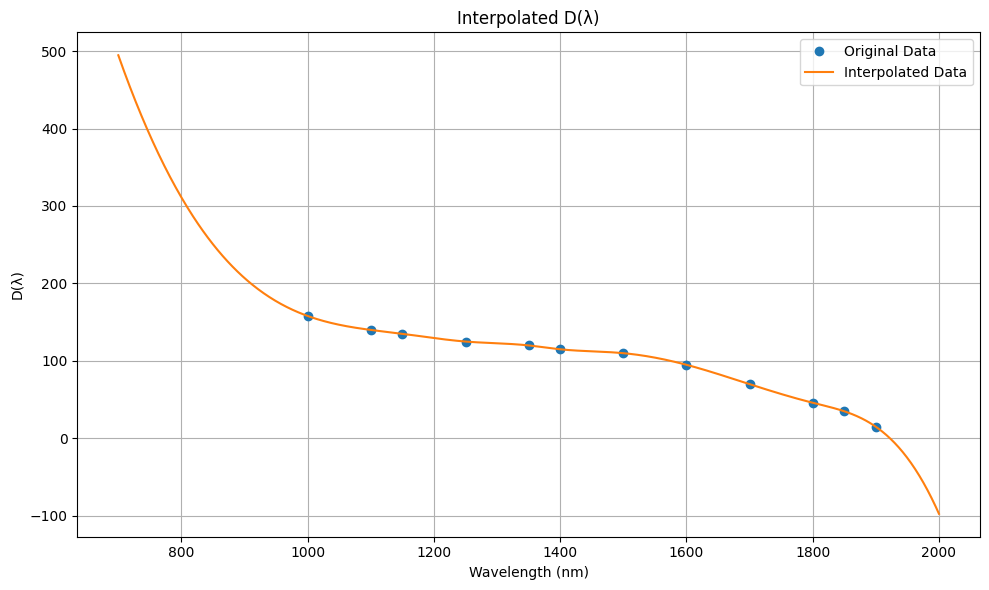
\includegraphics[width=0.9\linewidth]{D}
			\caption{Halogen lamp spectral radiation intensity}
			\label{fig:mereni}
		\end{figure}
		As we have acquired $D(\lambda)$ in the appropriate range, we can now use formula (3) to calculate the normalised response for both silicon and germanium. To get $S(\lambda)$ for both semiconductors, we again interpolate the measured data by a third-degree polynomial \footnote{Even though the third degree polynomial does not exactly copy the whole curve, it is a sufficient approximation. Higher degree polynomials would not change the result significantly}. The band gap $E_g$ is acquired by finding roots of these polynomials. We get data presented in Fig. 2.
		\begin{figure}[H]
			\centering
			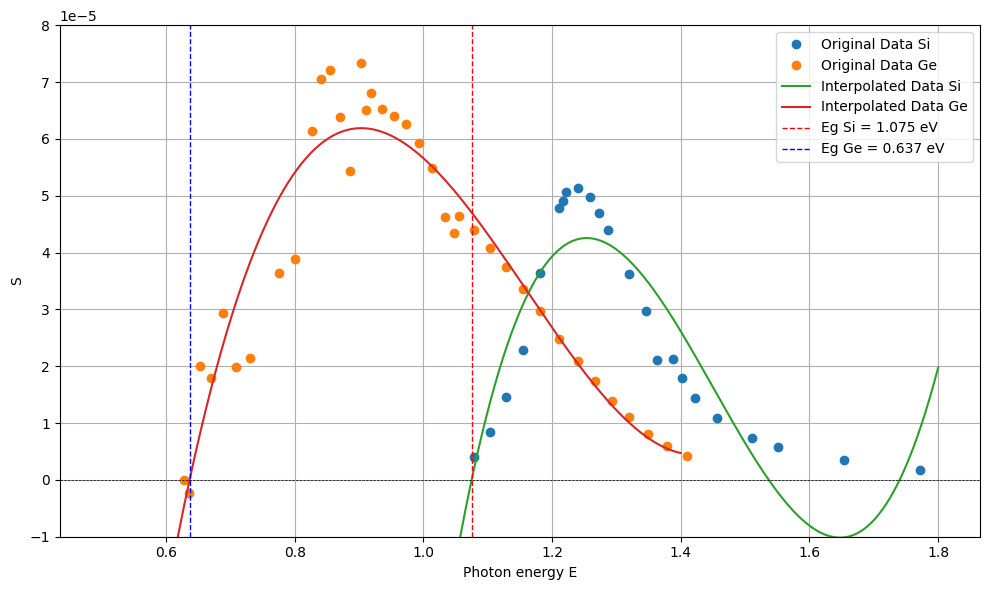
\includegraphics[width=0.9\linewidth]{results}
			\caption{Normalised photovoltage as a function of the light's energy.}
			\label{fig:mereni}
		\end{figure}
		To estimate the uncertainty of the extracted band gap energy $E_g$, we evaluated the standard deviation of residuals between the measured $S(E)$ values and the fitted polynomial:
		\[
		\sigma_S = \sqrt{\frac{1}{N} \sum_i \left[S_i - S_\text{fit}(E_i)\right]^2}
		\]
		
		The uncertainty of $E_g$ was then propagated using the slope of the fitted polynomial at the intersection point:
		\[
		\Delta E_g = \frac{\sigma_S}{\left| \frac{dS}{dE}(E_g) \right|}
		\]
		The band gap values are:
		\begin{gather*}
			E_{g_\mathrm{Ge}} = 0.64 \pm 0.19\,\mathrm{eV}\\
			E_{g_\mathrm{Si}} = 1.087 \pm 0.15 \,\mathrm{eV}
		\end{gather*}
	
		\section{Conclusion}
		Even though our measured data was affected by significant noise (especially measurements for Ge for energies lower than $1.0\, \mathrm{eV}$) which we are not able to explain, we have successfully acquired the band gap values for both silicon and germanium. By comparing our results to literature \cite{NIST}, we can see that our results are within satisfactory deviation from the real values. This deviation can be explained by our voltage measurement and monochromator resolution, the interpolation of the halogen lamp's spectral intensity distribution - we cannot be sure that the distribution is constant over the lamp's lifespan.
	
	\end{multicols}
		\section{Appendix - measured data}
		\begin{table}[H]
			\centering
			\begin{tabular}{rr|rr}
				\multicolumn{2}{c}{Germanium} & \multicolumn{2}{c}{Silicon}                 \\ \hline
				$\lambda \,\mathrm{[nm]}$     & $U \,\mathrm{[mV]}$     & $\lambda \,\mathrm{[nm]}$         & $U \,\mathrm{[mV]}$               \\ \hline
				880              & 0.930      & 700                  & 0.900                \\
				900              & 1.230      & 750                  & 1.350                \\
				920              & 1.560      & 800                  & 1.800                \\
				940              & 2.010      & 821                  & 2.100                \\
				960              & 2.400      & 852                  & 2.700                \\
				980              & 2.850      & 872                  & 3.300                \\
				1000             & 3.300      & 885                  & 3.900                \\
				1025             & 3.750      & 894                  & 4.500                \\
				1050             & 4.350      & 910                  & 4.200                \\
				1075             & 4.800      & 922                  & 5.700                \\
				1100             & 5.250      & 940                  & 6.600                \\
				1125             & 5.610      & 964                  & 7.500                \\
				1150             & 5.940      & 975                  & 7.800                \\
				1175             & 6.150      & 985                  & 8.100                \\
				1185             & 5.700      & 1000                 & 8.100                \\
				1200             & 6.000      & 1015                 & 7.800                \\
				1225             & 6.960      & 1020                 & 7.500                \\
				1250             & 7.410      & 1025                 & 7.260                \\
				1275             & 7.740      & 1050                 & 5.340                \\
				1300             & 7.860      & 1075                 & 3.270                \\
				1325             & 7.950      & 1100                 & 2.040                \\
				1350             & 8.160      & 1125                 & 1.170                \\
				1362.5           & 7.740      & 1150                 & 0.540                \\
				1375             & 8.610      & \multicolumn{1}{l}{} & \multicolumn{1}{l}{} \\
				1400             & 6.240      & \multicolumn{1}{l}{} & \multicolumn{1}{l}{} \\
				1425             & 7.230      & \multicolumn{1}{l}{} & \multicolumn{1}{l}{} \\
				1450             & 8.100      & \multicolumn{1}{l}{} & \multicolumn{1}{l}{} \\
				1475             & 7.860      & \multicolumn{1}{l}{} & \multicolumn{1}{l}{} \\
				1500             & 6.750      & \multicolumn{1}{l}{} & \multicolumn{1}{l}{} \\
				1550             & 4.050      & \multicolumn{1}{l}{} & \multicolumn{1}{l}{} \\
				1600             & 3.450      & \multicolumn{1}{l}{} & \multicolumn{1}{l}{} \\
				1700             & 1.500      & \multicolumn{1}{l}{} & \multicolumn{1}{l}{} \\
				1750             & 1.140      & \multicolumn{1}{l}{} & \multicolumn{1}{l}{} \\
				1800             & 1.350      & \multicolumn{1}{l}{} & \multicolumn{1}{l}{} \\
				1850             & 0.630      & \multicolumn{1}{l}{} & \multicolumn{1}{l}{} \\
				1900             & 0.300      & \multicolumn{1}{l}{} & \multicolumn{1}{l}{} \\
				1950             & 0.060      & \multicolumn{1}{l}{} & \multicolumn{1}{l}{} \\
				1975             & 0.000      & \multicolumn{1}{l}{} & \multicolumn{1}{l}{} \\ 
			\end{tabular}
		\end{table}

		

	\printbibliography
		
		
		% Nakonec nezapomeňte projet text programem vlna nebo vlnka, např.
		% 	vlna -m -l -n mojeuloha.tex
		% nebo zkontrolovat a opravit jednopísmenné předložky na koncích řádků ručně.
\end{document}
